\section{Deriva\c{c}\~oes em Fun\c{c}\~oes Mapeamento}\label{sec:derivative}
Para o exerc\'icio 4 tamb\'em foi utilizado o \textit{software} \texttt{Mathematica} para realizar os c\'alculos. A seguir a linha de pensamento base para o desenvolvimento do exerc\'icio.

Sabe-se que $x$ e $y$ s\~ao fun\c{c}\~oes diferenci\'aveis em $\xi$ e $\eta$. Com isso, os infinitesimais $d\xi$ e podem ser $d\eta$ transformado em $dx$ e $dy$ pela Eq. \eqref{eq:infinitesimal}.
\begin{equation}
    \begin{bmatrix}
        dx \\
        dy
    \end{bmatrix}
    =
    \begin{bmatrix}
        \frac{\partial x}{\partial \xi} & \frac{\partial x}{\partial \eta} \\
        \frac{\partial y}{\partial \xi} & \frac{\partial y}{\partial \eta}
    \end{bmatrix}
    \begin{bmatrix}
        d\xi\\
        d\eta
    \end{bmatrix}.
    \label{eq:infinitesimal}
\end{equation}

A matriz contendo as derivadas parciais da transforma\c{c}\~ao de coordenadas \'e chamada de matriz jacobiana ($Jac$). Invertendo o sistema de equa\c{c}\~oes da Eq. \eqref{eq:infinitesimal} tem-se a Eq. \eqref{eq:inverse}, usada para encontrar as derivadas parciais de $\xi$ e $\eta$ em fun\c{c}\~ao de $x$ e $y$.
\begin{equation}
    \begin{bmatrix}
        d\xi\\
        d\eta
    \end{bmatrix}
    =
    Jac^{-1}
    \begin{bmatrix}
        dx \\
        dy
    \end{bmatrix},
    \label{eq:inverse}
\end{equation}
sendo q o inverso da Jacobiana pode ser obtido conforme Eq. \eqref{eq:inverse_jac}.
\begin{equation}
    Jac^{-1} = \frac{1}{|Jac|}
    \begin{bmatrix}
        \frac{\partial y}{\partial \eta} & -\frac{\partial x}{\partial \eta} \\
        -\frac{\partial y}{\partial \xi} & \frac{\partial x}{\partial \xi}
    \end{bmatrix},
    \label{eq:inverse_jac}
\end{equation}
com $|Jac|$ sendo o determinante da matriz jacobiana dado pela Eq. \eqref{eq:determinant}.
\begin{equation}
    |Jac| = \frac{\partial x}{\partial \xi}\frac{\partial y}{\partial \eta} - \frac{\partial x}{\partial \eta}\frac{\partial y}{\partial \xi}.
    \label{eq:determinant}
\end{equation}

Plugando as eqs. \eqref{eq:inverse_jac} e \eqref{eq:determinant} na Eq. \eqref{eq:inverse} tem-se a Eq. \eqref{eq:finalMap}
\begin{equation}
    \label{eq:finalMap}
    \begin{cases}
        \frac{d\xi}{dx} =  \frac{1}{|Jac|}\frac{\partial y}{\partial \eta}\\
        \frac{d\eta}{dx} = -\frac{1}{|Jac|}\frac{\partial y}{\partial \xi}\\
        \frac{d\xi}{dy} = -\frac{1}{|Jac|}\frac{\partial x}{\partial \eta}\\
        \frac{d\eta}{dy} =  \frac{1}{|Jac|}\frac{\partial x}{\partial \xi}
    \end{cases}
\end{equation}

Finalmente, pode-se aplicar a regra da cadeia para encontrar o gradiente de $f$ com rela\c{c}\~ao a $\xi$ e $\eta$ em fun\c{c}\~ao de $x$ e $y$ conforme Eq. \eqref{eq:chainRule}.
\begin{equation}
    \label{eq:chainRule}
    \grad{\hat f} = 
    \begin{bmatrix}
        \frac{\partial \hat f}{\partial x} \\
        \frac{\partial \hat f}{\partial y}
    \end{bmatrix} = 
    \begin{bmatrix}
        \frac{\partial \hat f}{\partial \xi} \frac{\partial \xi }{dx} + \frac{\partial \hat f}{\partial \eta}\frac{\partial \eta}{dx}\\
        \frac{\partial \hat f}{\partial \xi} \frac{\partial \xi }{dy} + \frac{\partial \hat f}{\partial \eta}\frac{\partial \eta}{dy}
    \end{bmatrix}
\end{equation}

A partir da Eq. \eqref{eq:chainRule} pode-se calcular o gradiente de $\hat f$ em fun\c{c}\~ao de $\xi$ e $\eta$. A seguir, os resultados obtidos pelo c\'odigo em \texttt{Mathematica}. Real\c{c}a-se novamente que o c\'odigo na \'integra pode ser encontrado no Ap\^endice \ref{sec:github}.

Primeiramente, apresentam-se as derivadas parciais de $\hat f$ com rela\c{c}\~ao a $\xi$ e $\eta$
\begin{equation*}
    \begin{cases}
        \frac{d\hat f}{d\xi} = \frac{1}{4} (\eta -1) (-\eta -\xi -1)-\frac{1}{4} (\eta -1) (\xi -1) \\
        \frac{d\hat f}{d\eta} = \frac{1}{4} (\xi -1) (-\eta -\xi -1)-\frac{1}{4} (\eta -1) (\xi -1)  \\
    \end{cases},
\end{equation*}
as derivadas parciais de $x$ e $y$ com rela\c{c}\~ao a $\xi$ e $\eta$
\begin{equation*}
    \begin{cases}
        \frac{\partial x}{\partial \xi} = \frac{1}{4} (-2 \eta  \xi +2 \xi + 4) \\
        \frac{\partial x}{\partial \eta} = \frac{1}{4} \left(1-\xi ^2\right) \\
        \frac{\partial y}{\partial \xi} = \frac{1}{4} \left(1-\eta ^2\right) \\
        \frac{\partial y}{\partial \eta} = \frac{1}{4} (4-2 \eta  (\xi -1)) \\
    \end{cases}.
\end{equation*}
e o determinante da matriz jacobiana
\begin{equation*}
    |Jac| = \frac{1}{16} \left(\eta ^2 \left(3 \xi ^2-4 \xi +1\right)-4 \eta  \left(\xi ^2+3 \xi -2\right)+\xi ^2+8
    \xi +15\right)
\end{equation*}

Com os resultados das derivadas parciais, calcula-se o grdiente de $\hat f$. 
\begin{equation*}
    \frac{d\hat f}{dx} = \frac{2 (\eta -1) (\eta  (\xi -1)-2) (\eta +2 \xi )}{\eta ^2 \left(3 \xi ^2-4 \xi +1\right)-4 \eta 
    \left(\xi ^2+3 \xi -2\right)+\xi ^2+8 \xi +15}+\frac{1}{16} (\xi -1) \left(\xi ^2-1\right) (2 \eta
    +\xi )
\end{equation*}
\begin{equation*}
    \frac{d\hat f}{dy} = \frac{(\xi -1) \left(\eta ^2 (3 \xi -1)-\eta  (5 \xi +7)-2 \xi \right)}{\eta ^2 \left(3 \xi ^2-4 \xi
    +1\right)-4 \eta  \left(\xi ^2+3 \xi -2\right)+\xi ^2+8 \xi +15}
\end{equation*}

Por fim, apresenta-se na Fig. \ref{fig:grad4} o gr\'afico do gradiente de $\hat f$ em fun\c{c}\~ao de $x$ e $y$ e seu contorno no domínio.
\begin{figure}[H]
    \centering
    \subfloat[\label{fig:plotGradf4}]{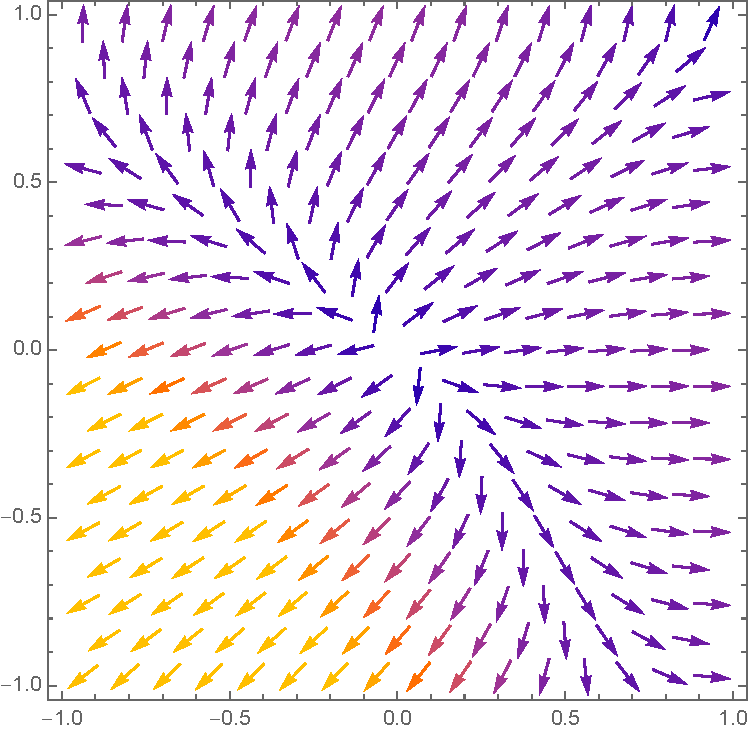
\includegraphics[width=0.49\textwidth]{Ex4GradF.pdf}}\hfill
    \subfloat[\label{fig:contourF4}]{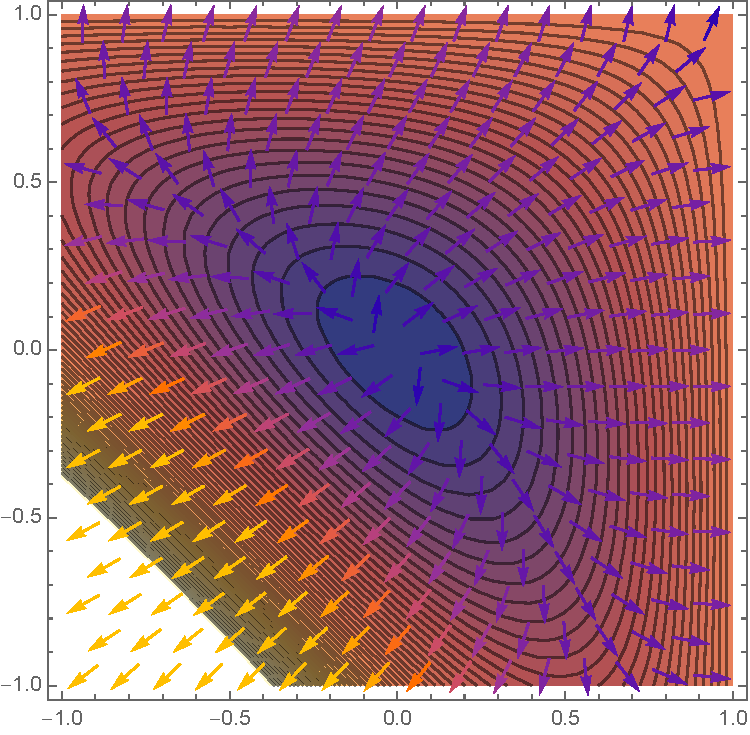
\includegraphics[width=0.49\textwidth]{Ex4ContourF.pdf}}
    \caption{Resultados: a) gradiente de $f$. b) Contorno de $\hat f$.}
    \label{fig:grad4}
\end{figure}